%!TEX root = JakubJedryszek2014.tex

\cleardoublepage


\chapter{AADL/BLESS to SPARK Ada Translation}
\label{codegen}

\begin{chapquote}{\textit{Randy Pausch}}
``Don’t complain; just work harder.''
\end{chapquote}


This chapter presents created AADL/BLESS to SPARK Ada translation schemes (\ref{codegen:mapping}), proposed port communication (\ref{codegen:port_communication}) and discusses design of an automatic translator, which can be created based on translation schemes (\ref{codegen:translator}).



\section{AADL/BLESS to SPARK Ada mapping}
\label{codegen:mapping}

%https://wiki.sei.cmu.edu/aadl/images/4/40/13_04_24-AADL-Code_Generation.pdf
%https://wiki.sei.cmu.edu/aadl/images/7/73/AADLV2Overview-AADLUserDay-Feb_2010.pdf (slide 35: port connections)

Mapping of AADL models to SPARK Ada is driven by "Architecture Analysis \& Design Language (AADL) V2 Programming Language Annex Document" \cite{AnnexDoc}. This document was discussed during AADL User Days in Valencia (February 2013)\footnote{http://www.aadl.info/aadl/downloads/committee/feb2013/presentations/13\_02\_04-AADL-Code\%20Generation.pdf} and in Jacksonville, FL (April 2013).\footnote{https://wiki.sei.cmu.edu/aadl/images/8/8a/Constraint\_Annex\_April22.v3.pdf} Ocarina tool suite (based on older AADL annex documents \cite{Ocarina:Article}) and its examples\footnote{https://github.com/yoogx/polyorb-hi-ada/tree/master/examples/aadlv2} were also helpful in understanding of AADL to Ada translation. Mapping of BLESS assertions was created in consultation with Brian Larson (BLESS creator).
 


\subsection{Data Types Mapping}
\label{codegen:mapping:data}

One of core AADL packages is \lstinline{Base_Types}. It defines fundamental data types for AADL. Its definition, without floating and text types, is shown in the Figure \ref{listing:aadl_base_types}. Every data type has a set of AADL properties (properties are used to define characteristics of an AADL component).

\begin{figure}%[ht]
\singlespacing
\begin{lstlisting}[language=aadl, frame=single, gobble=0]
package Base_Types
public
  with Data_Model;

  data Boolean
  properties 
    Data_Model::Data_Representation => Boolean;
  end Boolean;
  data Integer
  properties
    Data_Model::Data_Representation => Integer;
  end Integer;
  data Natural extends Integer
  properties 
    Data_Model::Integer_Range => 0 .. Max_Target_Integer;
  end Natural;
  data Integer_8 extends Integer
  properties
    Data_Model::Number_Representation => Signed;
    Source_Data_Size => 1 Bytes;
  end Integer_8;
  data Integer_16 extends Integer
  properties
    Data_Model::Number_Representation => Signed;
    Source_Data_Size => 2 Bytes;
  end Integer_16;
  data Integer_32 extends Integer
  properties
    Data_Model::Number_Representation => Signed;
    Source_Data_Size => 4 Bytes;
  end Integer_32;
  data Integer_64 extends Integer
  properties
    Data_Model::Number_Representation => Signed;
    Source_Data_Size => 8 Bytes;
  end Integer_64;
  data Unsigned_8 extends Integer
  properties
    Data_Model::Number_Representation => Unsigned;
    Source_Data_Size => 1 Bytes;
  end Unsigned_8;
  data Unsigned_16 extends Integer
  properties
    Data_Model::Number_Representation => Unsigned;
    Source_Data_Size => 2 Bytes;
  end Unsigned_16;
  data Unsigned_32 extends Integer
  properties
    Data_Model::Number_Representation => Unsigned;
    Source_Data_Size => 4 Bytes;
  end Unsigned_32;
  data Unsigned_64 extends Integer
  properties
    Data_Model::Number_Representation => Unsigned;
    Source_Data_Size => 8 Bytes;
  end Unsigned_64;  
end Base_Types;
\end{lstlisting} 
\doublespacing
\caption{AADL \lstinline{Base_Types} package}
\label{listing:aadl_base_types}
\end{figure}

In Ada 2012, and thus SPARK 2014, there is package \lstinline{Interfaces}, which allows for easy mapping of AADL \lstinline{Base_Types} package. The mapping proposed in Annex Document \cite{AnnexDoc} is presented in the Figure \ref{listing:aadl2spark2014_base_types_mapping}.

\begin{figure}%[ht]
\singlespacing
\begin{lstlisting}[language=aadl, frame=single, gobble=0]
with Interfaces;

package Base_Types is

	type AADL_Boolean is new Standard.Boolean;

	type AADL_Integer is new Standard.Integer;

	type AADL_Natural is new Standard.Integer;

 	type Integer_8 is new Interfaces.Integer_8;

 	type Integer_16 is new Interfaces.Integer_16;

	type Integer_32 is new Interfaces.Integer_32;

	type Integer_64 is new Interfaces.Integer_64;

	type Unsigned_8 is new Interfaces.Unsigned_8;

	type Unsigned_16 is new Interfaces.Unsigned_16;

	type Unsigned_32 is new Interfaces.Unsigned_32;

	type Unsigned_64 is new Interfaces.Unsigned_64;	

end Base_Types;
\end{lstlisting} 
\doublespacing
\caption{Mapping of \lstinline{Base_Types} for SPARK 2014}
\label{listing:aadl2spark2014_base_types_mapping}
\end{figure}

The target language for this thesis is SPARK 2005. We evaluated SPARK 2014, but determined that, at the time when this thesis was written SPARK 2014 tools were not mature enough and multitasking facilities were not yet included in the language. Types: \lstinline{Float}, \lstinline{Character} and \lstinline{String} are also not part of this thesis, because of the limitations of SPARK 2005 verification tools limitation. Thus, only \lstinline{Integer}, \lstinline{Enumeration}, \lstinline{Boolean} and \lstinline{Record} types are taken into account in mappings.

Each type is translated into simple type definition and protected type. Then it can be used in multitasking programs with the Ravenscar Profile. For every protected type only setter (\lstinline{Put}) and getter (\lstinline{Get}) subprograms are defined. The type can be extended by the developer during the development phase. Protected objects can be also removed if they are not needed. The default value for priority, for each generated type is 10. It can be changed during development phase to align with system goals. Types: \lstinline{Integer}, \lstinline{Boolean} and \lstinline{Natural} are already defined in SPARK Ada, thus only protected objects are generated for them. AADL \lstinline{Base_Types} mapping to SPARK 2005 is presented in the Table \ref{table:aadl2spark_types_simple}.

\singlespacing
\begin{center}
	\begin{longtable}{| p{2in} | p{4in} |}
	
		\caption{Base AADL types to SPARK mapping.}
		\label{table:aadl2spark_types_simple}
		\\
		\hline
		\multicolumn{1}{|c|}{\textbf{AADL}} & \multicolumn{1}{|c|}{\textbf{SPARK Ada}} \\ \hline
		\endfirsthead

		\multicolumn{2}{c}%
		{{\bfseries \tablename\ \thetable{} -- continued from previous page}} \\
		\hline 
		\multicolumn{1}{|c|}{\textbf{AADL}} & \multicolumn{1}{|c|}{\textbf{SPARK Ada}} \\ \hline
		\endhead

		\hline \multicolumn{2}{|r|}{{Continued on next page}} \\ \hline
		\endfoot

		\hline %\hline
		\endlastfoot

		\begin{lstlisting}[language=aadl]
			data Integer
			properties
				Data_Model::Data_Representation => Integer;
			end Integer;
		\end{lstlisting} 
		&
		\begin{lstlisting}[language=ada]
			protected type Integer_Store
		    is
		        pragma Priority (10);

		        function Get return Integer;
		        --# global in Integer_Store;

		        procedure Put(X : in Integer);
		        --# global out Integer_Store;
		        --# derives Integer_Store from X;
		    private
		        TheStoredData : Integer := 0;
		    end Integer_Store;
		\end{lstlisting} 

		\\ \hline

		\begin{lstlisting}[language=aadl]
			data Integer_16 extends Integer
			properties
				Data_Model::Number_Representation => Signed;
				Source_Data_Size => 2 Bytes;
			end Integer_16;
		\end{lstlisting} 
		&
		\begin{lstlisting}[language=ada]
			type Integer_16 is new Integer range -2**(2*8-1) .. 2**(2*8-1-1);

			protected type Integer_16_Store
		    is
		        pragma Priority (10);

		        function Get return Integer_16;
		        --# global in Integer_16_Store;

		        procedure Put(X : in Integer_16);
		        --# global out Integer_16_Store;
		        --# derives Integer_16_Store from X;
		    private
		        TheStoredData : Integer_16 := 0;
		    end Integer_16_Store;

		    protected body Integer_16_Store is
		        function Get return Integer_16
		        --# global in TheStoredData;
		        is
		        begin
		            return TheStoredData;
		        end Get;

		        procedure Put(X : in Integer_16)
		          --# global out TheStoredData;
		          --# derives TheStoredData from X;
		        is
		        begin
		            TheStoredData := X;
		        end Put;
		    end Integer_16_Store;
		\end{lstlisting} 

		\\ \hline

		\begin{lstlisting}[language=aadl]
			data Unsigned_16 extends Integer
			properties
				Data_Model::Number_Representation => Unsigned;
				Source_Data_Size => 2 Bytes;
			end Unsigned_16;
		\end{lstlisting} 
		&
		\begin{lstlisting}[language=ada]
			type Unsigned_16 is new Integer range 0 .. 2**(2*8-1);
    
		    protected type Unsigned_16_Store is pragma Priority (10);
			    function Get return Unsigned_16;
		        --# global in Unsigned_16_Store;
		        procedure Put(X : in Unsigned_16);
		        --# global out Unsigned_16_Store;
		        --# derives Unsigned_16_Store from X;
		    private
		        TheStoredData : Unsigned_16 := 0;
		    end Unsigned_16_Store;

		    protected body Unsigned_16_Store is
		        function Get return Unsigned_16
		        --# global in TheStoredData;
		        is begin 
		        	return TheStoredData; 
		        end Get;

		        procedure Put(X : in Unsigned_16)
		          --# global out TheStoredData;
		          --# derives TheStoredData from X;
		        is begin 
		        	TheStoredData := X; 
		        end Put;
		    end Unsigned_16_Store;
		\end{lstlisting}

		\\ \hline

		\begin{lstlisting}[language=aadl]
			data Type_With_Range
				properties
					Data_Model::Data_Representation => Integer;
					Data_Model::Base_Type => (classifier (Base_Types::Unsigned_16));
					Data_Model::Integer_Range => 0 .. 1000;
			end Type_With_Range;
		\end{lstlisting} 
		&
		\begin{lstlisting}[language=ada]
			type Type_With_Range is new Integer range 0 .. 1000;
    
		    protected type Type_With_Range_Store is pragma Priority (10);
			    function Get return Type_With_Range;
		        --# global in Type_With_Range_Store;
		        procedure Put(X : in Type_With_Range);
		        --# global out Type_With_Range_Store;
		        --# derives Type_With_Range_Store from X;
		    private
		        TheStoredData : Type_With_Range := 0;
		    end Unsigned_16_Store;

		    protected body Type_With_Range_Store is
		        function Get return Type_With_Range
		        --# global in TheStoredData;
		        is begin 
		        	return TheStoredData; 
		        end Get;

		        procedure Put(X : in Type_With_Range)
		          --# global out TheStoredData;
		          --# derives TheStoredData from X;
		        is begin 
		        	TheStoredData := X; 
		        end Put;
		    end Type_With_Range_Store;
		\end{lstlisting}
	\end{longtable}
\end{center}
\doublespacing

Type range is defined using AADL properties: \lstinline{Data_Model::Number_Representation}, \lstinline{Source_Data_Size} and \lstinline{Data_Model::Integer_Range}. When \lstinline{Data_Model::Integer_Range} property is not specified, then range is calculated. In case of \lstinline{Integer} representation, the range starts from negative value, for \lstinline{Unsigned} - from 0. The maximum value for \lstinline{Integer} is calculated using the formula \ref{eq:integer_max_formula}. 

\begin{equation} \label{eq:integer_max_formula}
	\text{Integer\_[Number\_Of\_Bytes * 8]\_Max} = 2^{\text{Number\_Of\_Bytes} * 8 - 1} - 1
\end{equation}

The minimum value formula for Integer (\ref{eq:integer_min_formula}) and maximum value for \lstinline{Unsigned} (\ref{eq:unsigned_max_formula}) use similar strategy.

\begin{equation} \label{eq:integer_min_formula}
	\text{Integer\_[Number\_Of\_Bytes * 8]\_Min} = -2^{\text{Number\_Of\_Bytes} * 8 - 1}
\end{equation}

\begin{equation} \label{eq:unsigned_max_formula}
	\text{Unsigned\_[Number\_Of\_Bytes * 8]\_Max} = 2^{\text{Number\_Of\_Bytes} * 8} - 1
\end{equation}

Mapping for enumeration types, presented in the Table \ref{table:aadl2spark_types_enums}, is straightforward. In addition to simple types, protected types are generated.

\singlespacing
\begin{center}
	\begin{longtable}{| p{3in} | p{3in} |}
	
		\caption{AADL enumeration types to SPARK mapping.}
		\label{table:aadl2spark_types_enums}
		\\
		\hline
		\multicolumn{1}{|c|}{\textbf{AADL}} & \multicolumn{1}{|c|}{\textbf{SPARK Ada}} \\ \hline
		\endfirsthead

		\multicolumn{2}{c}%
		{{\bfseries \tablename\ \thetable{} -- continued from previous page}} \\
		\hline 
		\multicolumn{1}{|c|}{\textbf{AADL}} & \multicolumn{1}{|c|}{\textbf{SPARK Ada}} \\ \hline
		\endhead

		\hline \multicolumn{2}{|r|}{{Continued on next page}} \\ \hline
		\endfoot

		\hline %\hline
		\endlastfoot

		\begin{lstlisting}[language=aadl]
			data Enum_Type
				properties
					Data_Model::Data_Representation => Enum;
					Data_Model::Enumerators => ("Enumerator1", "Enumerator2", "Enumerator3");
			end Enum_Type; 
		\end{lstlisting} 
		&
		\begin{lstlisting}[language=ada]
			type Enum_Type is (Enumerator1, Enumerator2, Enumerator3);

			protected type Enum_Type_Store
		    is
		        pragma Priority (10);

		        function Get return Enum_Type;
		        --# global in Enum_Type_Store;

		        procedure Put(X : in Enum_Type);
		        --# global out Enum_Type_Store;
		        --# derives Enum_Type_Store from X;
		    private
		        TheStoredData : Enum_Type := Enum_Type'First;
		    end Enum_Type_Store;

		    protected body Enum_Type_Store is
		        function Get return Enum_Type
		        --# global in TheStoredData;
		        is
		        begin
		            return TheStoredData;
		        end Get;

		        procedure Put(X : in Enum_Type)
		          --# global out TheStoredData;
		          --# derives TheStoredData from X;
		        is
		        begin
		            TheStoredData := X;
		        end Put;
		    end Enum_Type_Store;
		\end{lstlisting} 
			
	\end{longtable}
\end{center}
\doublespacing

Sometimes it is pragmatic to define a type that has exactly the same range as an already existing type, especially when it is used for some specific calculations, e.g., measuring speed. Let's say, that \lstinline{Unsigned_16} was used. Then, during development of next car model, when a larger number of bits are required to hold anticipated values, it becomes not enough. In case when e.g., \lstinline{Speed_Type} is not defined, there are two possible resolutions. First: change definition (range) of \lstinline{Unsigned_16}. That is bad choice, especially because its name specify the range. Another reason: it might be used not only for measuring the Speed, but maybe also for fuel level, which range is still fine. Second option is to change \lstinline{Unsigned_16} to e.g. \lstinline{Unsigned_32} everywhere in Speed Control Module (and maybe also in some external modules). When \lstinline{Speed_Type} is defined and used everywhere for speed units, then only definition of \lstinline{Speed_Type} has to be changed. To define type, which is an extension to already existing type in AADL, \lstinline{extends} clause has to be used. To create, new type, which is based on existing type \lstinline{Data_Model::Base_Type} property has to be used. There are two ways to define type based on some other type in SPARK Ada:

\begin{itemize}
	\item subtype - it is compatible with its parent, in other words: parent type variable can be assigned to it, if its value is in the subtype range
	\item derived type - it is incompatible with its parent (parent type variable cannot be assigned to it), but inherits its primitive operations
\end{itemize}

Translation of AADL type created by extension of existing type to SPARK Ada subtype and AADL type created using \lstinline{Data_Model::Base_Type} property to SPARK Ada derived type is shown in the Table \ref{table:aadl2spark_types_subtypes}.

\singlespacing
\begin{center}
	\begin{longtable}{| p{3in} | p{3in} |}
	
		\caption{AADL types to SPARK mapping: Subtypes.}
		\label{table:aadl2spark_types_subtypes}
		\\
		\hline
		\multicolumn{1}{|c|}{\textbf{AADL}} & \multicolumn{1}{|c|}{\textbf{SPARK Ada}} \\ \hline
		\endfirsthead

		\multicolumn{2}{c}%
		{{\bfseries \tablename\ \thetable{} -- continued from previous page}} \\
		\hline 
		\multicolumn{1}{|c|}{\textbf{AADL}} & \multicolumn{1}{|c|}{\textbf{SPARK Ada}} \\ \hline
		\endhead

		\hline \multicolumn{2}{|r|}{{Continued on next page}} \\ \hline
		\endfoot

		\hline %\hline
		\endlastfoot

		\begin{lstlisting}[language=aadl]
			data Speed_Type extends Base_Types::Integer
			end Speed_Type;
		\end{lstlisting} 
		&
		\begin{lstlisting}[language=ada]
			subtype Speed_Type is Base_Types.Integer;
		\end{lstlisting} 

		\\
		\hline
		\begin{lstlisting}[language=aadl]
			data Speed_Type
			 	properties
			 		Data_Model::Base_Type => (classifier(Base_Types::Unsigned_16));
			end Speed_Type;
		\end{lstlisting} 
		&
		\begin{lstlisting}[language=ada]
			type Speed_Type is new Base_Types.Unsigned_16;
		\end{lstlisting} 
		
			
	\end{longtable}
\end{center}
\doublespacing

\newpage

AADL array type can be defined using property \lstinline{Data_Model::Data_Representation}. In addition to that, size for array has to be specified by \lstinline{Data_Model::Dimension} property. Sample mapping of array of 10 integers is shown in the Table \ref{table:aadl2spark_types_arrays}.

\singlespacing
\begin{center}
	\begin{longtable}{| p{3in} | p{3in} |}
	
		\caption{AADL arrays to SPARK Ada mapping}
		\label{table:aadl2spark_types_arrays}
		\\
		\hline
		\multicolumn{1}{|c|}{\textbf{AADL}} & \multicolumn{1}{|c|}{\textbf{SPARK Ada}} \\ \hline
		\endfirsthead

		\multicolumn{2}{c}%
		{{\bfseries \tablename\ \thetable{} -- continued from previous page}} \\
		\hline 
		\multicolumn{1}{|c|}{\textbf{AADL}} & \multicolumn{1}{|c|}{\textbf{SPARK Ada}} \\ \hline
		\endhead

		\hline \multicolumn{2}{|r|}{{Continued on next page}} \\ \hline
		\endfoot

		\hline %\hline
		\endlastfoot

		\begin{lstlisting}[language=aadl]
			data Some_Array
			  	properties
			  		Data_Model::Data_Representation => Array;
				    Data_Model::Base_Type => (classifier(Base_Types::Integer_32));
				    Data_Model::Dimension => (10);
			end Some_Array;
		\end{lstlisting} 
		&
		\begin{lstlisting}[language=ada]
			subtype Some_Array_Index is Integer range 1 .. 10;
    		type Some_Array is array (Some_Array_Index) of Base_Types.Integer_32;

    		protected type Some_Array_Store
		    is
		        pragma Priority (10);

		        function Get(Ind : in Integer) return Base_Types.Integer_32;
		        --# global in Some_Array_Store;

		        procedure Put(Ind : in Integer; Val : in Base_Types.Integer_32);
		        --# global in out Some_Array_Store;
		        --# derives Some_Array_Store from Some_Array_Store, Ind, Val;
		    private
		        TheStoredData : Some_Array := Some_Array'(others => 0);
		    end Some_Array_Store;

		    protected body Some_Array_Store
		    is
		        function Get(Ind : in Integer) return Base_Types.Integer_32
		        --# global in TheStoredData;
		        is
		        begin
		            return TheStoredData(Ind);
		        end Get;

		        procedure Put(Ind : in Integer; Val : in Base_Types.Integer_32)
		          --# global in out TheStoredData;
		          --# derives TheStoredData from TheStoredData, Ind, Val;
		        is
		        begin
		            TheStoredData(Ind) := Val;
		        end Put;
		    end Some_Array_Store;
		\end{lstlisting} 
			
	\end{longtable}
\end{center}
\doublespacing

AADL v2 allows to create struct data types, using \lstinline{Data_Model::Data_Representation => Struct}. AADL Struct is mapped to SPARK Ada record type. The mapping is presented in the Table \ref{table:aadl2spark_types_records}.

\singlespacing
\begin{center}
	\begin{longtable}{| p{3in} | p{3in} |}
	
		\caption{AADL struct to SPARK Ada record mapping}
		\label{table:aadl2spark_types_records}
		\\
		\hline
		\multicolumn{1}{|c|}{\textbf{AADL}} & \multicolumn{1}{|c|}{\textbf{SPARK Ada}} \\ \hline
		\endfirsthead

		\multicolumn{2}{c}%
		{{\bfseries \tablename\ \thetable{} -- continued from previous page}} \\
		\hline 
		\multicolumn{1}{|c|}{\textbf{AADL}} & \multicolumn{1}{|c|}{\textbf{SPARK Ada}} \\ \hline
		\endhead

		\hline \multicolumn{2}{|r|}{{Continued on next page}} \\ \hline
		\endfoot

		\hline %\hline
		\endlastfoot

		\begin{lstlisting}[language=aadl]
			data Some_Record_Type
				properties
					Data_Model::Data_Representation => Struct;
					Data_Model::Element_Names => ("Field1", "Field2", "Field3");
					Data_Model::Base_Type => 
					( 
						classifier(Base_Types::Integer_32), 			    
						classifier(Base_Types::Boolean),
						classifier(Base_Types::Unsigned_32)
					);      
			end Some_Record_Type;  
		\end{lstlisting} 
		&
		\begin{lstlisting}[language=ada]
			type Some_Record_Type is record
		        Field1 : Integer_32;
		        Field2 : Boolean;
		        Field3 : Unsigned_32;
		    end record;
		\end{lstlisting} 
			
	\end{longtable}
\end{center}
\doublespacing

Data types translations are created based on Brian Larson's AADL/BLESS models of PCA Pump. They are syntacticly verified with SPARK Examiner. During development of types mapping, SPARK Examiner was helpful also for detecting inconsistencies in AADL models, e.g., it detected redundancy in enumerators. Both \lstinline{Alarm_Type} and \lstinline{Warning_Type} contained \lstinline{No_Alarm} enumerator, which was a bug. All enumerators, for all types have to be unique. Thus, \lstinline{Warning_Type} should have \lstinline{No_Warning} enumerator instead.


\subsection{AADL Ports Mapping}
\label{codegen:mapping:ports}

The proposed ports mapping shown in the Table \ref{table:aadl2spark_ports} is based on AADL runtime services from Annex 2 to "Programming Language Annex Document" \cite{AnnexDoc}. Additionally, the mapping contains SPARK 2005 contracts, i.e., \lstinline{global} and \lstinline{derives} annotations to denote global variables usage and variable dependencies. Data types used by ports has to be defined earlier, to be visible. Moreover, for port communication, protected types are used, to enable concurrency. Simple types are denoted as \lstinline{Port_Type}, while their protected equivalents as \lstinline{Port_Type_Store}. Proposed mapping assume single-process application. In order to create distributed system, middle-ware layer has to be created to assure ports communication.

% maybe split right column into 2 rows: spec and body?
\singlespacing
\begin{center}
	\begin{longtable}{| p{2in} | p{4in} |}
	
		\caption{AADL to SPARK Ada ports mapping.}
		\label{table:aadl2spark_ports}
		\\
		\hline
		\multicolumn{1}{|c|}{\textbf{AADL}} & \multicolumn{1}{|c|}{\textbf{SPARK Ada}} \\ \hline
		\endfirsthead

		\multicolumn{2}{c}%
		{{\bfseries \tablename\ \thetable{} -- continued from previous page}} \\
		\hline 
		\multicolumn{1}{|c|}{\textbf{AADL}} & \multicolumn{1}{|c|}{\textbf{SPARK Ada}} \\ \hline
		\endhead

		\hline \multicolumn{2}{|r|}{{Continued on next page}} \\ \hline
		\endfoot

		\hline %\hline
		\endlastfoot

		\begin{lstlisting}[language=aadl]
			Port_Name : 
				in data port Port_Type;
		\end{lstlisting} 
		&
		\begin{lstlisting}[language=ada]
			-- spec (.ads):
			--# own protected Port_Name : Port_Type_Store(Priority => 10)

			procedure Receive_Port_Name;
			--# global out Port_Name;

			-- body (.adb):
			Port_Name : Port_Type_Store;

			procedure Receive_Port_Name
			is
			begin
				-- TODO: implement receiving Port_Name value
				-- e.g.:
				-- Port_Name.Put(Some_Pkg.Get_Port_Name)
			end Receive_Port_Name;
		\end{lstlisting} 

		\\ \hline

		\begin{lstlisting}[language=aadl]
			Port_Name : 
				out data port Port_Type;
		\end{lstlisting} 
		&
		\begin{lstlisting}[language=ada]
			-- spec (.ads)
			--# own protected Port_Name : Port_Type_Store(Priority => 10)
			
			procedure Get_Port_Name(Port_Name_Out : out Port_Type);
			--# global in Port_Name;
			--# derives Port_Name_Out from Port_Name;

			-- body (.adb):
			Port_Name : Port_Type_Store;

			procedure Get_Port_Name(Port_Name_Out : out Port_Type)
			is
			begin
				Port_Name_Out := Port_Name.Get;
			end Get_Port_Name;
		\end{lstlisting} 

		\\ \hline

		\begin{lstlisting}[language=aadl]
			Port_Name : 
				in event port;
		\end{lstlisting} 
		&
		\begin{lstlisting}[language=ada]
			-- spec (.ads)
			procedure Put_Port_Name;

			-- body (.adb):
			procedure Put_Port_Name 
			is
			begin
				-- TODO: implement event handler
			end Put_Port_Name;
		\end{lstlisting} 

		\\ \hline

		\begin{lstlisting}[language=aadl]
			Port_Name : 
				out event port;
		\end{lstlisting} 
		&
		\begin{lstlisting}[language=ada]
			-- spec (.ads)
			procedure Send_Port_Name;

			-- body (.adb):

			procedure Send_Port_Name 
			is
			begin
				-- TODO: implement sending event
				-- e.g.:
				-- Some_Pkg.Put_Port_Name;
			end Send_Port_Name;
		\end{lstlisting} 

		\\ \hline

		\begin{lstlisting}[language=aadl]
			Port_Name : 
				in event data port Port_Type;
		\end{lstlisting} 
		&
		\begin{lstlisting}[language=ada]
			-- spec (.ads)
			procedure Put_Port_Name(Port_Name_In : Port_Type);

			-- body (.adb):
			procedure Put_Port_Name (Port_Name_In : Port_Type) 
			is
			begin
				-- TODO: implement data event handler
			end Put_Port_Name;
		\end{lstlisting} 

		\\ \hline

		\begin{lstlisting}[language=aadl]
			Port_Name : 
				out event data port Port_Type;
		\end{lstlisting} 
		&
		\begin{lstlisting}[language=ada]
			-- spec (.ads)			
			procedure Send_Port_Name;

			-- body (.adb):
			procedure Send_Port_Name 
			is
			begin
				-- TODO: implement sending event data
				-- e.g.:
				-- Some_Pkg.Put_Port_Name(Port_Name);
			end Send_Port_Name;
		\end{lstlisting} 
	\end{longtable}
\end{center}
\doublespacing


\subsection{Thread to Task Mapping}
\label{codegen:mapping:threads}

AADL Threads to SPARK Ada tasks mapping proposed in this thesis is presented in the Table \ref{table:threads2tasks}. Communication between threads is described in Section \ref{codegen:port_communication:thread}.

\singlespacing
\begin{table}[!ht]
	\caption{AADL threads to SPARK Ada tasks mapping.}
	\label{table:threads2tasks}
	\centering
  	\begin{tabular}{ | p{3.5in} | p{2.5in} |}

		\hline
		\multicolumn{1}{|c|}{\textbf{AADL}} & \multicolumn{1}{|c|}{\textbf{SPARK Ada}} \\ \hline

		\begin{lstlisting}[language=aadl]
			package Some_Pkg
				thread Some_Thread
					features
						Some_Port : out data port Port_Type;
				end Some_Thread;

				thread implementation Some_Thread.imp
				end Some_Thread.imp;
			end Some_Pkg;
		\end{lstlisting} 
		& 
		\begin{lstlisting}
			package Some_Pkg
			is
				task type Some_Thread
				--# global out Some_Port;
				is
					pragma Priority(10);
				end Some_Thread;
			end Some_Pkg;

			package body Some_Pkg
			is
				st : Some_Thread;

				task body Some_Thread
				is
				begin
					loop
						-- implementation
					end loop;
				end Some_Thread;
			end Some_Pkg;
		\end{lstlisting} 

		\\ \hline
	\end{tabular}
\end{table}
\doublespacing


\subsection{Subprograms Mapping}
\label{codegen:mapping:subprograms}

The mapping of subprograms is also straightforward. However, in our proposal it is different than the mapping proposed in "AADL Code Generation Annex" \cite{AnnexDoc}. Flexibility realized by translating appropriate AADL properties is not needed in approach presented in this thesis. Thus \lstinline{renames} clause is not needed, because it is taken form subprogram name in AADL model. The \lstinline{Source_Language} property is also not needed, because only one language in targeted (SPARK Ada). For now, the body of subprogram is empty, because behavior (implementation) is not supported by proposed translator. Subprogram mapping should be revised and consulted with AADL committee members, in order to understand their design decisions.

\singlespacing
\begin{table}[!ht]
	\caption{AADL subprograms to SPARK Ada subprograms mapping.}
	\label{table:subprograms_mapping}
	\centering
  	\begin{tabular}{ | p{3in} | p{3in} |}

		\hline
		\multicolumn{1}{|c|}{\textbf{AADL}} & \multicolumn{1}{|c|}{\textbf{SPARK Ada}} \\ \hline

		\begin{lstlisting}[language=aadl]
			subprogram sp
			features
				e : in parameter T;
				s : out parameter T;
			end sp;
		\end{lstlisting} 
		& 
		\begin{lstlisting}
			procedure sp(e : in T; s : out T);

			procedure sp(e : in T; s : out T) is 
			begin
				--# implementation
			end sp;
		\end{lstlisting} 		

		\\ \hline
	\end{tabular}
\end{table}
\doublespacing


\subsection{Feature Groups Mapping}
\label{codegen:mapping:feature_groups}

In SPARK Ada there are nested packages and child packages. Sample nested packages are shown in the Figure \ref{listing:nested_packages}. Equivalent child packages are shown in the Figure \ref{listing:child_packages}. The name of a child package consists of the parent unit's name followed by the child package's identifier, separated by a period (dot) '.'. Calling convention is the same for child and nested packages (e.g. \lstinline{P.N} in figures \ref{listing:nested_packages} and \ref{listing:child_packages}). However, there is a difference between nested packages and child packages. In nested package, declarations become visible as they are introduced, in textual order. For example, in the Figure \ref{listing:nested_packages} spec \lstinline{N} cannot refer to \lstinline{M} in any way. In case of child packages, with certain exceptions, all the functionality of the parent is available to a child and parent can access all its child packages. More precisely: all public and private declarations of the parent package are visible to all child packages. Private child package can be accessed only from parent's body.

\begin{figure}[ht]
\singlespacing
\begin{lstlisting}[language=ada, frame=single, gobble=0]
package P is
   D: Integer;

   --  a nested package:
   package N is
      X: Integer;
   private
      Foo: Integer;
   end N;

   E: Integer;
private
   --  nested package in private section:
   package M is
      Y: Integer;
   private
      Bar: Integer;
   end M;

end P;
\end{lstlisting}
\doublespacing
\caption{Nested packages in SPARK Ada}
\label{listing:nested_packages}
\end{figure}

\begin{figure}[ht]
\singlespacing
\begin{lstlisting}[language=ada, frame=single, gobble=0]
package P is
   D: Integer;
   E: Integer;
end P;

package P.N is 	-- a child package
  X: Integer;
private
  Foo: Integer;
end P.N;

private package P.M is 	-- a child private package
  Y: Integer;
private
  Bar: Integer;
end P.M;
\end{lstlisting}
\doublespacing
\caption{Child packages in SPARK Ada}
\label{listing:child_packages}
\end{figure}

\clearpage

The thesis author identified a possible approach to create child package and encapsulate one feature group in it. However, SPARK Ada does not allow to access a child package's private part from its parent. Thus, the proposed approach would require to expose feature group internal variables as public, which is undesirable. Thus, a feature group is translated with prefix \lstinline{Feature_Group_Name_*}. Feature group mapping is presented in Section \ref{codegen:mapping:packages}, in figures \ref{listing:aadl_sample}, \ref{listing:package_mapping_spec} and \ref{listing:package_mapping_body}. In essence, the feature group is "flatten", i.e., the encapsulation feature of feature groups is removed and elements of feature groups are uniquely identified by using the feature group name as a prefix.


\subsection{AADL Package to SPARK Ada Package Mapping}
\label{codegen:mapping:packages}

Figure \ref{listing:aadl_sample} presents a sample AADL package with a \lstinline{system} component. It contains all the categories of ports described in Section \ref{codegen:mapping:ports} as well as one feature group with two ports as example of feature group mapping.

\begin{figure}[ht]
\singlespacing
\begin{lstlisting}[language=aadl, frame=single, gobble=0]
package Some_Pkg
public
with Base_Types;

feature group Some_Features
features
  Some_Out_Port: out data port Base_Types::Integer;
  Some_In_Port: in data port Base_Types::Integer;
end Some_Features;

system Some_System
features
  Some_Feature_Group : feature group Some_Features;
  
  In_Data_Port : in data port Base_Types::Integer;
  Out_Data_Port : out data port Base_Types::Integer;
  In_Event_Port : in event port;
  Out_Event_Port : out event port;
  In_Event_Data_Port : in event data port Base_Types::Integer;
  Out_Event_Data_Port : out event data port Base_Types::Integer;
end Some_System;

end Some_Pkg;
\end{lstlisting}
\doublespacing
\caption{Sample AADL package with system}
\label{listing:aadl_sample}
\end{figure}

For now, only single process SPARK Ada application is considered. Thus, ports are exposed only on the system level. Communication between threads in process will be realized by protected objects and only SPARK annotations and data types will be needed as described in Section \ref{codegen:mapping:threads}. Based on the ports mapping presented in Section \ref{codegen:mapping:ports}, the translation to a SPARK Ada package is shown in the Figure \ref{listing:package_mapping_spec} and Figure \ref{listing:package_mapping_body}. 

\begin{figure}[ht]
\singlespacing
\begin{lstlisting}[language=ada, frame=single, gobble=0]
package Some_Pkg
--# own Some_Features_Some_Out_Port : Integer;
--#     Some_Features_Some_In_Port : Integer;
--#     In_Data_Port : Integer;
--#     Out_Data_Port : Integer;
--# initializes Some_Features_Some_Out_Port,
--#             Some_Features_Some_In_Port,
--#             In_Data_Port,
--#             Out_Data_Port;
is

    function Some_Features_Get_Some_Out_Port return Integer;
    --# global in Some_Features_Some_Out_Port;

    procedure Some_Features_Receive_Some_In_Port;
    --# global out Some_Features_Some_In_Port;

    procedure Receive_In_Data_Port;
    --# global out In_Data_Port;

    function Get_Out_Data_Port return Integer;
    --# global in Out_Data_Port;

    procedure Put_In_Event_Port;

    procedure Send_Out_Event_Port;

    procedure Put_In_Event_Data_Port(In_Event_Data_Port_In : Integer);

    procedure Send_Out_Event_Data_Port;

end Some_Pkg;
\end{lstlisting}
\doublespacing
\caption{Translation of sample AADL package from Figure \ref{listing:aadl_sample} - package specification}
\label{listing:package_mapping_spec}
\end{figure}

\begin{figure}[ht]
\singlespacing
\begin{lstlisting}[language=ada, frame=single, gobble=0]
package body Some_Pkg
is
    Some_Features_Some_Out_Port : Integer := 0;
    Some_Features_Some_In_Port : Integer := 0;
    In_Data_Port : Integer := 0;
    Out_Data_Port : Integer := 0;

    function Some_Features_Get_Some_Out_Port return Integer
    is
    begin
        return Some_Features_Some_Out_Port;
    end Some_Features_Get_Some_Out_Port;

    procedure Some_Features_Receive_Some_In_Port
    is
    begin
        -- implementation
    end Some_Features_Receive_Some_In_Port;

    procedure Receive_In_Data_Port
    is
    begin
        -- implementation
    end Receive_In_Data_Port;

    function Get_Out_Data_Port return Integer
    is
    begin
        return Out_Data_Port;
    end Get_Out_Data_Port;

    procedure Put_In_Event_Port
    is
    begin
        -- implementation
    end Put_In_Event_Port;

    procedure Send_Out_Event_Port
    is
    begin
        -- implementation
    end Send_Out_Event_Port;

    procedure Put_In_Event_Data_Port(In_Event_Data_Port_In : Integer)
    is
    begin
        -- implementation
    end Put_In_Event_Data_Port;

    procedure Send_Out_Event_Data_Port
    is
    begin
        -- implementation
    end Send_Out_Event_Data_Port;

end Some_Pkg;
\end{lstlisting}
\doublespacing
\caption{Translation of sample AADL package from Figure \ref{listing:aadl_sample} - package body}
\label{listing:package_mapping_body}
\end{figure}



\subsection{AADL Property Set to SPARK Ada Package Mapping}
\label{codegen:mapping:propertyset}

In the AADL property set, new properties, types and constants can be defined. There is no equivalent construct in SPARK Ada. Thus property set is mapped to SPARK Ada package. In this thesis, only properties of type \lstinline{constant aadlinteger} are considered. There are issues with using non-constant types in SPARK Ada package (e.g. when using them in some type definition). Table \ref{table:propertyset_mapping} shows sample property set mapping to SPARK Ada package.

\singlespacing
\begin{table}[!ht]
	\caption{AADL property set to SPARK Ada package mapping}
	\label{table:propertyset_mapping}
	\centering
  	\begin{tabular}{ | p{3in} | p{3in} |}

		\hline
		\multicolumn{1}{|c|}{\textbf{AADL}} & \multicolumn{1}{|c|}{\textbf{SPARK Ada}} \\ \hline

		\begin{lstlisting}[language=aadl]
			property set Some_Properties 
			is
				Some_Property1 : constant aadlinteger => 10 applies to (all);
				Some_Property2 : constant aadlinteger => 27 applies to (all);
				Some_Property3 : constant aadlinteger => Some_Properties::Some_Property1 applies to (all);
			end Some_Properties;
		\end{lstlisting} 
		& 
		\begin{lstlisting}
			package Some_Properties
			is
				Some_Property1 : constant Integer := 10;
				Some_Property2 : constant Integer := 27;
				Some_Property3 : constant Integer := Some_Property1;
			end Some_Properties;
		\end{lstlisting} 		

		\\ \hline
	\end{tabular}
\end{table}
\doublespacing

In AADL, all declarations must have an \lstinline{applies to} clause, which indicates the model element(s) to which a property is assigned. It is ignored in the target of the translation. However, future version of the translator might use it, e.g., for automatic generation of \lstinline{with} clauses or could be translated to comments (to inform developer about modeling assumptions).


\subsection{BLESS Mapping}
\label{codegen:mapping:bless}

In cooperation with Brian Larson, translations for BLESS assertions, invariant, pre- and postconditions were created. Table \ref{table:bless2spark} presents their mapping to SPARK Ada. Generated (translated) code may not be complete. In such situations, developer effort to implement missing parts will be required, e.g., when assertion is specified in AADL/BLESS model, but not defined, it has to be implemented in SPARK Ada.

\singlespacing
\begin{center}
	\begin{longtable}{| p{3in} | p{3in} |}
		\caption{BLESS to SPARK contracts mapping}
		\label{table:bless2spark}
		\\
		\hline
		\multicolumn{1}{|c|}{\textbf{AADL/BLESS}} & \multicolumn{1}{|c|}{\textbf{SPARK Ada}} \\ \hline
		\endfirsthead

		\multicolumn{2}{c}%
		{{\bfseries \tablename\ \thetable{} -- continued from previous page}} \\
		\hline 
		\multicolumn{1}{|c|}{\textbf{AADL/BLESS}} & \multicolumn{1}{|c|}{\textbf{SPARK Ada}} \\ \hline
		\endhead

		\hline \multicolumn{2}{|r|}{{Continued on next page}} \\ \hline
		\endfoot

		\hline %\hline
		\endlastfoot

		\begin{lstlisting}[language=bless]
			BLESS::Assertion=>"<<COND1()>>"
		\end{lstlisting} 
		& 
		\begin{lstlisting}
			--# assert COND1;
		\end{lstlisting} 

		\\ \hline

		\begin{lstlisting}[language=bless]
			thread Some_Thread
			features
				Some_Port : out event port
				{BLESS::Assertion => "<<(Var1 < Var2 and COND2())>>";};
			end Some_Thread;
		\end{lstlisting} 
		& 
		\begin{lstlisting}
			task body Some_Thread
			is
			begin
				loop
					--# assert (Var1 < Var2 and COND2);
				end loop;
			end Some_Thread;
		\end{lstlisting} 

		\\ \hline

		\begin{lstlisting}[language=bless]
			thread implementation Some_Thread.imp
			annex BLESS 
			{**
				invariant <<(Some_Var < Other_Var)>>
			**};
			end Some_Thread.imp;
		\end{lstlisting} 
		& 
		\begin{lstlisting}
			task body Some_Thread
			is
			begin
				loop
					--# assert (Some_Var < Other_Var);
				end loop;
			end Some_Thread;
		\end{lstlisting} 

		\\ \hline

		\begin{lstlisting}[language=bless]
			thread implementation Some_Thread.imp
			annex BLESS 
			{**
				assert
				<<State1 : :COND1() or COND2()>>
				<<Var : :=
  								(State1()) -> 0,
  								(State2()) -> -1,
  								(State3()) -> 9
				>>
			**};
			end Some_Thread.imp;
		\end{lstlisting} 
		& 
		\begin{lstlisting}
			task body Some_Thread
			is
			begin
				loop
					--# assert (COND1 or COND2)
					--#          -> State1();
					--# assert (Var = 0) -> State1 and
					--#        (Var = -1) -> State2 and
					--#        (Var = 9) -> State3;
				end loop;
			end Some_Thread;
		\end{lstlisting} 

		\\ \hline

		\begin{lstlisting}[language=bless]
			subprogram Some_Subprogram
			features 
				param : out parameter Base_Types::Integer;
			annex subBless
			{**
				pre <<(param > 0)>>
				post <<(param = 0)>>
			**};
			end Some_Subprogram;
		\end{lstlisting} 
		& 
		\begin{lstlisting}
			procedure Some_Subprogram(Param : in out Integer);
		    --# pre Param > 0;
		    --# post Param = 0;
		\end{lstlisting} 
		
	\end{longtable}
\end{center}
\doublespacing

\clearpage

\section{Port-based Communication}
\label{codegen:port_communication}

Communication between AADL components is realized by ports. AADL ports can be declared in subprograms, threads, processes, systems and other entities. In this Section, communication between threads in a single-process SPARK Ada application (\ref{codegen:port_communication:thread}) and concepts of communication between two systems (\ref{codegen:port_communication:system}) are presented. 


\subsection{Threads Communication}
\label{codegen:port_communication:thread}

\begin{wrapfigure}{r}{0.4\textwidth}
    \begin{center}
    	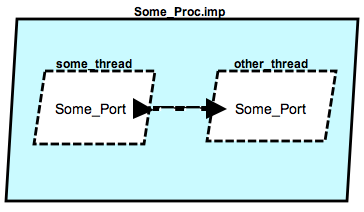
\includegraphics[width=0.4\textwidth]{figures/port-communication-thread.png}
    \end{center}
    \caption{Example of port communication between threads}
    \label{figure:port_communication_thread}
\end{wrapfigure}

An example of communication between threads in a single process is depicted in Figure \ref{figure:port_communication_thread}. There are two threads (\lstinline{some_thread} and \lstinline{other_thread}) in one process. The AADL model and its translation to SPARK Ada are presented in the Table \ref{table:port_communication_thread}. The connection between threads has to be specified in the process implementation. Based on the mappings from Section \ref{codegen:mapping}, a protected object is defined, but subprograms are not, because communication takes place only internally. Thus, subprograms are not necessary. The result of translation consists of two tasks and a private global protected object, which enables communication between them. Additionally, both tasks have global annotations (one with \lstinline{out} mode, other with \lstinline{in} mode), which indicate the use of a protected object in their bodies.

\begin{table} %[!ht]
	\caption{Translation of AADL threads communication to SPARK Ada}
	\label{table:port_communication_thread}
	\singlespacing
	\centering
  	\begin{tabular}{ | p{3in} | p{3in} |}

		\hline
		\multicolumn{1}{|c|}{\textbf{AADL}} & \multicolumn{1}{|c|}{\textbf{SPARK Ada}} \\ \hline

		\begin{lstlisting}[language=aadl]
			package Some_Pkg
			public
			with Base_Types;

				process Some_Proc
				end Some_Proc;
				
				process implementation Some_Proc.imp
				subcomponents
					some_thread: thread Some_Thread.imp;
					other_thread: thread Other_Thread.imp;
				connections
					connection: port some_thread.Some_Port -> other_thread.Some_Port;
				end Some_Proc.imp;

				thread Some_Thread
					features
						Some_Port : out data port Base_Types::Integer;
				end Some_Thread;

				thread implementation Some_Thread.imp
				end Some_Thread.imp;
				
				thread Other_Thread
					features
						Some_Port : in data port Base_Types::Integer;
				end Other_Thread;

				thread implementation Other_Thread.imp
				end Other_Thread.imp;
							
			end Some_Pkg;
		\end{lstlisting} 
		& 
		\begin{lstlisting}
			with Base_Types;
			--# inherit Base_Types;
			package Some_Pkg
			--# own task st : Some_Thread;
			--#     task ot : Other_Thread;
			--#     protected Some_Port : Base_Types.Integer_Store (Priority => 10);
			is
			   
			private   
			   task type Some_Thread     
			   --# global out Some_Port;   
			   is
			      pragma Priority (10);
			   end Some_Thread;
			   
			   task type Other_Thread
			   --# global in Some_Port;
			   is      
			      pragma Priority (10);      
			   end Other_Thread;	   
			end Some_Pkg;

			package body Some_Pkg
			is
			   st : Some_Thread;
			   ot : Other_Thread;
			   Some_Port : Base_Types.Integer_Store;

			   task body Some_Thread is begin      
			      loop         
			         -- implementation
			      end loop;      
			   end Some_Thread;
			   
			   task body Other_Thread is begin      
			      loop
			         -- implementation       
			      end loop;      
			   end Other_Thread;   
			end Some_Pkg;	
		\end{lstlisting} 		

		\\ \hline
	\end{tabular}
\end{table}
\doublespacing

Threads can be also placed in different packages. The same example of two threads within one process, but in different packages is presented in the Table \ref{table:port_communication_thread_different_pkg}. In this case, subprograms present in mapping table, in Section \ref{codegen:port_communication} are also present in resulted translation. Moreover, body of procedure \lstinline{Receive_Some_Port} is implemented as a result of defined connection between threads in the process implementation, in AADL model.

\singlespacing
\begin{center}
	\begin{longtable}{| p{2in} | p{4in} |}
	
		\caption{AADL threads communication to SPARK Ada tasks communication translation (multiple packages)}
		\label{table:port_communication_thread_different_pkg}
		\\
		\hline
		\multicolumn{1}{|c|}{\textbf{AADL}} & \multicolumn{1}{|c|}{\textbf{SPARK Ada}} \\ \hline
		\endfirsthead

		\multicolumn{2}{c}%
		{{\bfseries \tablename\ \thetable{} -- continued from previous page}} \\
		\hline 
		\multicolumn{1}{|c|}{\textbf{AADL}} & \multicolumn{1}{|c|}{\textbf{SPARK Ada}} \\ \hline
		\endhead

		\hline \multicolumn{2}{|r|}{{Continued on next page}} \\ \hline
		\endfoot

		\hline %\hline
		\endlastfoot

		\begin{lstlisting}[language=aadl]
			package Pkg1
			public
			with Base_Types, Pkg2;

				process Some_Proc
				end Some_Proc;
				
				process implementation Some_Proc.imp
				subcomponents
					some_thread: thread Some_Thread.imp;
					other_thread: thread Pkg2::Other_Thread.imp;
				connections
					connection: port some_thread.Some_Port -> other_thread.Some_Port;
				end Some_Proc.imp;

				thread Some_Thread
					features
						Some_Port : out data port Base_Types::Integer;
				end Some_Thread;

				thread implementation Some_Thread.imp
				end Some_Thread.imp;
		\end{lstlisting} 
		& 
		\begin{lstlisting}
			with Base_Types;
			--# inherit Base_Types;
			package Pkg1
			--# own task st : Some_Thread;
			--#     protected Some_Port : Base_Types.Integer_Store (Priority => 10);
			is
			   procedure Get_Some_Port(Some_Port_Out : out Integer);
			   --# global in Some_Port;
			   --# derives Some_Port_Out from Some_Port;
			   
			private   
			   task type Some_Thread     
			   --# global out Some_Port;   
			   is
			      pragma Priority (10);
			   end Some_Thread;
			end Pkg1;

			package body Pkg1
			is
			   st : Some_Thread;
			   Some_Port : Base_Types.Integer_Store;
			   
			   procedure Get_Some_Port(Some_Port_Out : out Integer)
			   is
			   begin
			      Some_Port_Out := Some_Port.Get;
			   end Get_Some_Port;
			      
			   task body Some_Thread
			   is   
			   begin      
			      loop         
			         -- implementation
			      end loop;      
			   end Some_Thread;

			end Pkg1;
		\end{lstlisting} 		

		\\ \hline

		\begin{lstlisting}[language=aadl]
			package Pkg2
			public
			with Base_Types;

				thread Other_Thread
					features
						Some_Port : in data port Base_Types::Integer;
				end Other_Thread;

				thread implementation Other_Thread.imp
				end Other_Thread.imp;
			end Pkg2;
		\end{lstlisting} 
		& 
		\begin{lstlisting}
			with Base_Types;
			with Pkg1;
			--# inherit Base_Types,
			--#         Pkg1;
			package Pkg2
			--# own task ot : Other_Thread;
			--#     protected Some_Port : Base_Types.Integer_Store(Priority => 10);
			is
			   procedure Receive_Some_Port;
			   --# global out Some_Port;
			   --#        in Pkg1.Some_Port;
			   
			private   
			   task type Other_Thread
			   --# global in Some_Port;
			   is      
			      pragma Priority (10);      
			   end Other_Thread;
			end Pkg2;

			package body Pkg2
			is
			   ot : Other_Thread;
			   Some_Port : Base_Types.Integer_Store;
			   
			   procedure Receive_Some_Port 
			   is
			      Temp : Integer;
			   begin
			      Pkg1.Get_Some_Port(Temp);
			      Some_Port.Put(Temp);
			   end Receive_Some_Port;   
			   
			   task body Other_Thread 
			   is 
			   begin
			      loop         
			         -- implementation
			      end loop;      
			   end Other_Thread;
			end Pkg2;
		\end{lstlisting} 
	\end{longtable}
\end{center}
\doublespacing

\clearpage

In the given example, communication is one way: from \lstinline{Pkg1} package to \lstinline{Pkg2} package. Thus, \lstinline{Pkg1} package does not need to know that \lstinline{Pkg2} package exists. In other words: it does not need to "with" it. However, if two way communication is needed (between \lstinline{Pkg1} to \lstinline{Pkg2}), then \lstinline{Pkg1} package has to "with" \lstinline{Pkg2} package. Note that no "with" is needed in the first example (Table \ref{table:port_communication_thread}), where communication between threads take place in the same package. A modified model of second example, with communication from \lstinline{Pkg2} to \lstinline{Pkg1}, is depicted in the Figure \ref{figure:port_communication_thread_two_way} and presented in the Figure \ref{listing:port_communication_thread_two_way}. 

\begin{figure}[h] %{r}{0.5\textwidth}%t=top, b=bottom, h=here
    \begin{center}
    	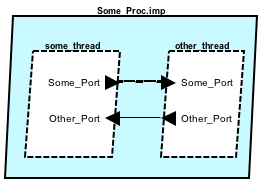
\includegraphics[width=0.5\textwidth]{figures/port-communication-thread-two-way.png}
    \end{center}
    \caption{Example of two way port communication between threads in different packages}
    \label{figure:port_communication_thread_two_way}
\end{figure}

\begin{figure}[ht]
\singlespacing
\begin{lstlisting}[language=aadl, frame=single, gobble=0]
package Pkg1TwoWay
public
with Base_Types, 
     Pkg2TwoWay;

	process Some_Proc
	end Some_Proc;	

	process implementation Some_Proc.imp
	subcomponents
		some_thread: thread Some_Thread.imp;
		other_thread: thread Pkg2TwoWay::Other_Thread.imp;
	connections
		connection: port some_thread.Some_Port -> other_thread.Some_Port;
		connection2: port some_thread.Other_Port -> other_thread.Other_Port;
	end Some_Proc.imp;

	thread Some_Thread
	features
		Some_Port : out data port Base_Types::Integer;
		Other_Port : in data port Base_Types::Integer;
	end Some_Thread;

	thread implementation Some_Thread.imp
	end Some_Thread.imp;	

end Pkg1TwoWay;

package Pkg2TwoWay
public
with Base_Types;

	thread Other_Thread
	features
		Some_Port : in data port Base_Types::Integer;
		Other_Port : out data port Base_Types::Integer;
	end Other_Thread;

	thread implementation Other_Thread.imp
	end Other_Thread.imp;

end Pkg2TwoWay;
\end{lstlisting} 
\doublespacing
\caption{AADL model of two way port communication threads in different packages}
\label{listing:port_communication_thread_two_way}
\end{figure}

This model, translated to SPARK Ada is presented in the Figure \ref{listing:port_communication_thread_two_way_spark_pkg1twoway} and Figure \ref{listing:port_communication_thread_two_way_spark_pkg2twoway}. It will not compile. GNAT compiler returns \lstinline{circular unit dependency} error. Additionally verification with SPARK Examiner returns error: \lstinline{Semantic Error 135 - The package Pkg2TwoWay is undeclared or not visible, or there is a circularity in the list of inherited packages}. Now, the problem is that two-way communication is allowed in AADL, but not in SPARK, nor even in Ada. Finding an appropriate solution requires further investigation, which is omitted in this thesis.

\begin{figure}[ht]
\singlespacing
\begin{lstlisting}[language=ada, frame=single, gobble=0]
with Base_Types;
with Pkg2TwoWay;
--# inherit Base_Types,
--#         Pkg2TwoWay;
package Pkg1TwoWay
--# own task st : Some_Thread;
--#     protected Some_Port : Base_Types.Integer_Store (Priority => 10);
--#     protected Other_Port : Base_Types.Integer_Store (Priority => 10);
is
   procedure Get_Some_Port(Some_Port_Out : out Integer);
   --# global in Some_Port;
   --# derives Some_Port_Out from Some_Port;
   
   procedure Receive_Other_Port;
   --# global out Other_Port;
   --#        in Pkg2TwoWay.Other_Port;
   
private   
   task type Some_Thread     
   --# global out Some_Port;   
   is
      pragma Priority (10);
   end Some_Thread;
end Pkg1TwoWay;

package body Pkg1TwoWay
is
   st : Some_Thread;
   Some_Port : Base_Types.Integer_Store;
   Other_Port : Base_Types.Integer_Store;
   
   procedure Get_Some_Port(Some_Port_Out : out Integer)
   is
   begin
      Some_Port_Out := Some_Port.Get;
   end Get_Some_Port;
   
   procedure Receive_Other_Port
   is
      Temp : Integer;
   begin
      Pkg2TwoWay.Get_Other_Port(Temp);
      Other_Port.Put(Temp);
   end Receive_Other_Port;
      
   task body Some_Thread
   is   
   begin      
      loop         
         -- implementation
         null;         
      end loop;      
   end Some_Thread;

end Pkg1TwoWay;
\end{lstlisting} 
\doublespacing
\caption{Two way port communication translated to SPARK Ada: package \lstinline{Pkg1TwoWay}}
\label{listing:port_communication_thread_two_way_spark_pkg1twoway}
\end{figure}

\begin{figure}[ht]
\singlespacing
\begin{lstlisting}[language=ada, frame=single, gobble=0]
with Base_Types;
with Pkg1TwoWay;
--# inherit Base_Types,
--#         Pkg1TwoWay;
package Pkg2TwoWay
--# own task ot : Other_Thread;
--#     protected Some_Port : Base_Types.Integer_Store (Priority => 10);
--#     protected Other_Port : Base_Types.Integer_Store (Priority => 10);
is
   procedure Receive_Some_Port;
   --# global out Some_Port;
   --#        in Pkg1TwoWay.Some_Port;

   procedure Get_Other_Port(Other_Port_Out : out Integer);
   --# global in Other_Port;
   --# derives Other_Port_Out from Other_Port;

private
   task type Other_Thread
   --# global in Some_Port;
   is
      pragma Priority (10);
   end Other_Thread;
end Pkg2TwoWay;

package body Pkg2TwoWay
is
   ot : Other_Thread;
   Some_Port : Base_Types.Integer_Store;
   Other_Port : Base_Types.Integer_Store;
   
   procedure Receive_Some_Port
   is
      Temp : Integer;
   begin
      Pkg1TwoWay.Get_Some_Port(Temp);
      Some_Port.Put(Temp);
   end Receive_Some_Port;   
   
   procedure Get_Other_Port(Other_Port_Out : out Integer)
   is
   begin
      Other_Port_Out := Other_Port.Get;
   end Get_Other_Port;
   
   task body Other_Thread
   is   
   begin      
      loop         
         -- implementation
         null;         
      end loop;      
   end Other_Thread;

end Pkg2TwoWay;
\end{lstlisting} 
\doublespacing
\caption{Two way port communication translated to SPARK Ada: package \lstinline{Pkg2TwoWay}}
\label{listing:port_communication_thread_two_way_spark_pkg2twoway}
\end{figure}

\clearpage

\subsection{Systems Communication}
\label{codegen:port_communication:system}

This Section provides a proposal for handling communication between different systems. An AADL system consists of process(es), and process consists of threads. Ports would be exposed by a package if they are specified in system entity. Communication between two systems can be described by another system. Figure \ref{figure:port_communication} presents communication between two systems: panel and pump. AADL model of this system comprises 3 packages: \lstinline{Main}, \lstinline{Panel} and \lstinline{Pump}. They are presented in the figures \ref{listing:port_communication_panel}, \ref{listing:port_communication_pump} and \ref{listing:port_communication_main}. The \lstinline{Panel} package has one thread \lstinline{Panel_Thread} with two \lstinline{out} ports: \lstinline{event port} and \lstinline{event data port}. Both ports are exposed by the process \lstinline{panel_process} and then by system \lstinline{panel}. \lstinline{Pump} package has similar structure, but two \lstinline{in} ports. Both are also exposed by process (\lstinline{pump_process}) and system (\lstinline{pump}). Connections between these two packages are defined in \lstinline{Main} package.

\begin{figure}[h] %{r}{0.6\textwidth}%[ht]%t=top, b=bottom, h=here
    \begin{center}
    	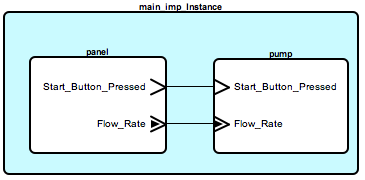
\includegraphics[width=0.7\textwidth]{figures/port-communication.png}    	
    \end{center}
    \caption{Example of port communication between systems}
    \label{figure:port_communication}
\end{figure}

\begin{figure} %[ht]
\singlespacing
\begin{lstlisting}[language=aadl, frame=single, gobble=0]
package Panel
public
with Base_Types;

	thread Panel_Thread
	features
		Start_Button_Pressed: out event port;
		Flow_Rate: out event data port Base_Types::Integer;
	end Panel_Thread;
	
	thread implementation Panel_Thread.imp
	end Panel_Thread.imp;
	
	process panel_process
		features
			Start_Button_Pressed: out event port;
			Flow_Rate: out event data port Base_Types::Integer;
	end panel_process;
	
	process implementation panel_process.imp
		subcomponents
			panel_thread: thread Panel_Thread.imp;
		connections
			sbp: port panel_thread.Start_Button_Pressed->Start_Button_Pressed;
			fr: port panel_thread.Flow_Rate->Flow_Rate;
	end panel_process.imp;
	
	system panel
		features 
			Start_Button_Pressed: out event port;
			Flow_Rate: out event data port Base_Types::Integer;
	end panel;
	
	system implementation panel.imp
		subcomponents
			panel_process: process panel_process.imp;
		connections
			sbp: port panel_process.Start_Button_Pressed->Start_Button_Pressed;
			fr: port panel_process.Flow_Rate->Flow_Rate;
	end panel.imp;
	
end Panel;
\end{lstlisting} 
\doublespacing
\caption{AADL model of port communication between systems: package \lstinline{Panel}}
\label{listing:port_communication_panel}
\end{figure}

\begin{figure}%[ht]
\singlespacing
\begin{lstlisting}[language=aadl, frame=single, gobble=0]
package Pump
public
with Base_Types;
	thread Rate_Controller
		features 
			Start_Button_Pressed: in event port;
			Flow_Rate: in event data port Base_Types::Integer;
	end Rate_Controller;	
	thread implementation Rate_Controller.imp
	end Rate_Controller.imp;
	
	process pump_process
		features
			Start_Button_Pressed : in event port;
			Flow_Rate: in event data port Base_Types::Integer;
	end pump_process;	
	process implementation pump_process.imp
		subcomponents
			Rate_Controller: thread Rate_Controller.imp;
		connections		
			sbp: port Start_Button_Pressed->Rate_Controller.Start_Button_Pressed;
			fr: port Flow_Rate->Rate_Controller.Flow_Rate;
	end pump_process.imp;
	
	system pump
		features
			Start_Button_Pressed : in event port;
			Flow_Rate: in event data port Base_Types::Integer;
	end pump;	
	system implementation pump.imp
		subcomponents
			pump_process : process pump_process.imp;
		connections
			sbp: port Start_Button_Pressed->pump_process.Start_Button_Pressed;
			fr: port Flow_Rate->pump_process.Flow_Rate;
	end pump.imp;
end Pump;
\end{lstlisting} 
\doublespacing
\caption{AADL model of port communication between systems: package \lstinline{Pump}}
\label{listing:port_communication_pump}
\end{figure}

\begin{figure}%[ht]
\singlespacing
\begin{lstlisting}[language=aadl, frame=single, gobble=0]
package Main
public
with Pump, Panel;
	system main	
	end main;	
	system implementation main.imp
		subcomponents
			panel: system Panel::panel.imp;
			pump: system Pump::pump.imp;
		connections
			sbp2sbp: port panel.Start_Button_Pressed->pump.Start_Button_Pressed;
			fr2fr: port panel.Flow_Rate->pump.Flow_Rate;
	end main.imp;
end Main;
\end{lstlisting} 
\doublespacing
\caption{AADL model of port communication between systems: package \lstinline{Main}}
\label{listing:port_communication_main}
\end{figure}

\clearpage

Based on mappings from Section \ref{codegen:mapping}, conforming SPARK Ada code is presented in the figures \ref{listing:port_communication_spark_panel} and \ref{listing:port_communication_spark_pump}. There are two packages: \lstinline{Panel} and \lstinline{Pump}. \lstinline{Main} package is omitted. Both contain procedures representing port interfaces, according to ports mapping from Section \ref{codegen:mapping:ports}. There is mocked port communication between event data ports. Each package has local variable, which are updated in case of event action. Additionally, procedures responsible for port communication consist appropriate annotations (i.e., \lstinline{global} and \lstinline{derives}). Translator should generate this code in case when connection between ports is specified in AADL model. Both packages consist of empty thread declarations and bodies, which conforms to translations from Section \ref{codegen:mapping:threads}. However, in this case, both packages will work in different systems, thus different processes. To enable communication between different systems, deployment methodology and the middle-ware layer has to be created. It will be used to enable not only system to system communication, but also communication with devices. This requires significant effort and was not needed for PCA Pump Prototype created in this thesis, thus it is considered as part of future work described in chapter \ref{future_work}.

\begin{figure}[ht]
\singlespacing
\begin{lstlisting}[language=ada, frame=single, gobble=0]
with Pump;
with Base_Types;
--# inherit Pump,
--#         Base_Types;
package Panel
--# own task pt : Panel_Thread;
--#     protected Flow_Rate : Base_Types.Integer_Store (Priority => 10);
is
    procedure Send_Start_Button_Pressed;

    procedure Send_Flow_Rate;
    --# global in Flow_Rate;
    --#        out Pump.Flow_Rate;

private
    task type Panel_Thread
    --# global in out Flow_Rate;
    is
        pragma Priority (10);
    end Panel_Thread;

end Panel;

package body Panel
is
    pt : Panel_Thread;
    Flow_Rate : Base_Types.Integer_Store;

    procedure Send_Start_Button_Pressed
    is begin
        Pump.Put_Start_Button_Pressed;
    end Send_Start_Button_Pressed;

    procedure Send_Flow_Rate
    is
        Flow_Rate_Temp : Integer;
    begin
        Flow_Rate_Temp := Flow_Rate.Get;
        Pump.Put_Flow_Rate(Flow_Rate_Temp);
    end Send_Flow_Rate;

    task body Panel_Thread
    is begin
      loop
         -- implementation
      end loop;      
    end Panel_Thread;
end Panel;
\end{lstlisting} 
\doublespacing
\caption{Port communication translated to SPARK Ada: package \lstinline{Panel}}
\label{listing:port_communication_spark_panel}
\end{figure}

\begin{figure}[ht]
\singlespacing
\begin{lstlisting}[language=ada, frame=single, gobble=0]
with Base_Types;
--# inherit Base_Types;
package Pump
--# own task rc : Rate_Controller;
--#     protected Flow_Rate : Base_Types.Integer_Store (Priority => 10);
is
    procedure Put_Start_Button_Pressed;

    procedure Put_Flow_Rate(Flow_Rate_In : Integer);
    --# global out Flow_Rate;
    --# derives Flow_Rate from Flow_Rate_In;

private
    task type Rate_Controller
    --# global in out Flow_Rate;
    is
        pragma Priority (10);
    end Rate_Controller;
end Pump;

package body Pump
is
    rc : Rate_Controller;
    Flow_Rate : Base_Types.Integer_Store;

    procedure Put_Start_Button_Pressed
    is
    begin
        -- TODO: implement event handler
    end Put_Start_Button_Pressed;

    procedure Put_Flow_Rate(Flow_Rate_In : Integer)
    is
    begin
        Flow_Rate.Put(Flow_Rate_In);
    end Put_Flow_Rate;

    task body Rate_Controller
    is
    begin
      loop
         -- implementation
        end loop;
    end Rate_Controller;
end Pump;
\end{lstlisting} 
\doublespacing
\caption{Port communication translated to SPARK Ada: package \lstinline{Pump}}
\label{listing:port_communication_spark_pump}
\end{figure}

\clearpage


\section{Towards an Automatic Translator}
\label{codegen:translator}

The ultimate goal is to create translator, which performs translations described in \ref{codegen:mapping} and \ref{codegen:port_communication} automatically. An automatic translator should enable either translation of entire model or parts of the model. An initial implementation strategy might focus on supporting only a subset of AADL entities: the system, process, thread, subprogram and port communication. The following functions should be supported:
\begin{itemize}
	\item data types translation (as described in Section \ref{codegen:mapping:data})
	\item threads to tasks translation (as described in \ref{codegen:mapping:threads})
	\item single ports translation (based on Section \ref{codegen:mapping:ports})
	\item subprogram to procedure/function translation (based on Section \ref{codegen:mapping:subprograms})
	\item single package translation with system, which contains ports and feature groups (as described in Section \ref{codegen:mapping:packages})
	\item property set mapping to SPARK Ada package (like in Section \ref{codegen:mapping:propertyset})
\end{itemize}

A possible second step would be to introduce BLESS support, specifically, add supported BLESS constructs described in Section \ref{codegen:mapping:bless}:
\begin{itemize}
	\item assertions for threads
	\item pre- and postconditions for subprograms
\end{itemize}

The recommended way to create translator is to parse AADL models, create Abstract Syntax Tree (AST), and emit code using the Visitor pattern. A parser and AST can be generated using ANTLR\footnote{http://www.antlr.org/} (Another Tool for Language Recognition) and its grammar development environment ANTLRWorks.\footnote{http://tunnelvisionlabs.com/products/demo/antlrworks} ANTLR 4 (with ANTLRWorks 2) enables automatic AST creation and handles left recursion, which makes parser development much easier and faster. Another tool, Xtext\footnote{http://www.eclipse.org/Xtext/index.html} can be also used (instead of ANTLR) for parser and AST generator. For emitting code, StringTemplate\footnote{http://www.stringtemplate.org/} (template engine for generating code) can be used. 

Development should be performed incrementally -- starting from the translation for the simplest constructs, like data types or single ports, and ending with port communication and BLESS support. First step, would be AADL grammar development. It is recommended to initially specify only the part of required AADL subset and then extend it incrementally. During translator development, unit testing and Test Driven Development is recommended. Translation schemes can be used as input and expected output of particular test cases. This will help to ensure correctness of translator while working on new features support.

Additionally, the automatic translator should work in two modes:
\begin{itemize}
	\item Ravenscar: as described above, with protected objects and multiple tasks
	\item Sequential: single-threaded application, without notion of tasks and protected objects	
\end{itemize}
